\exercise[Robot Vision]

\subsection{Description of joint estimation algorithm}


\subsection{Comparing estimations with sinusoidal signals}
\begin{center}
    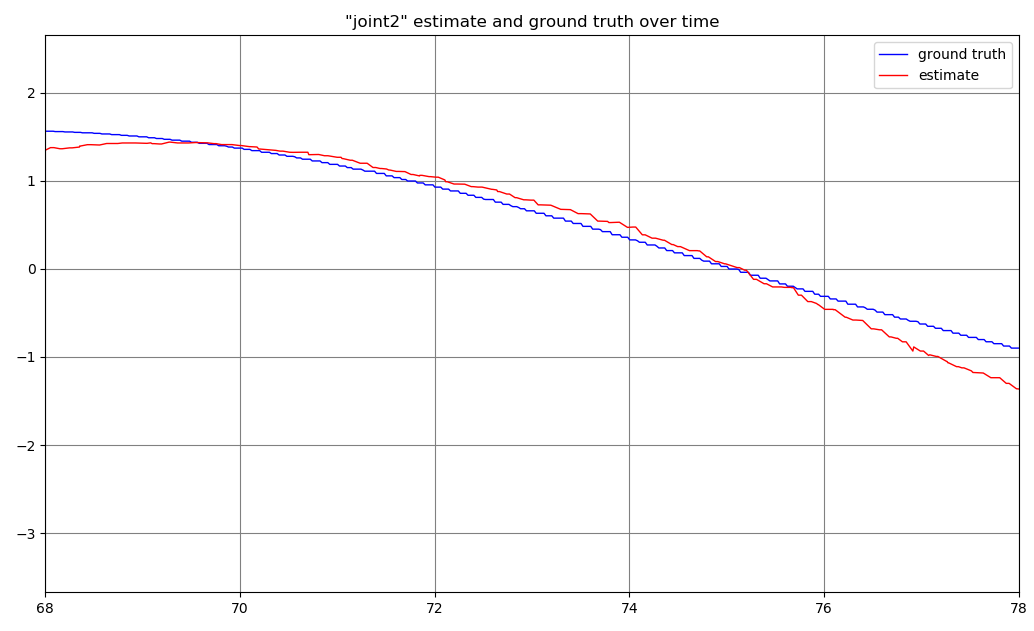
\includegraphics[width=0.7\textwidth]{plots/q2_1_j2_10sec.png}
    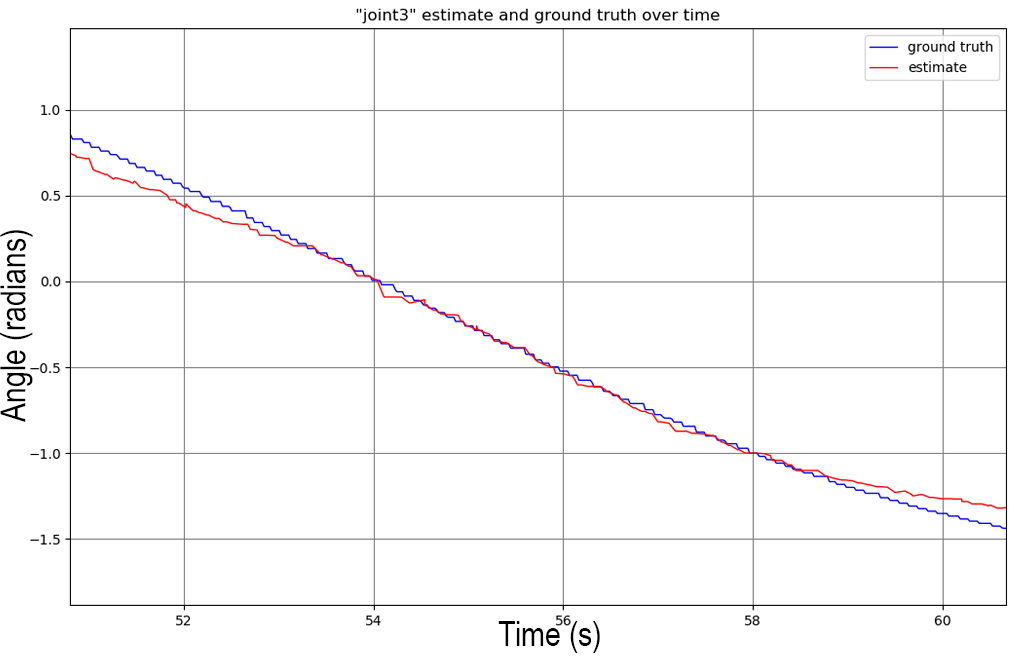
\includegraphics[width=0.7\textwidth]{plots/q2_1_j3_10sec.png}
    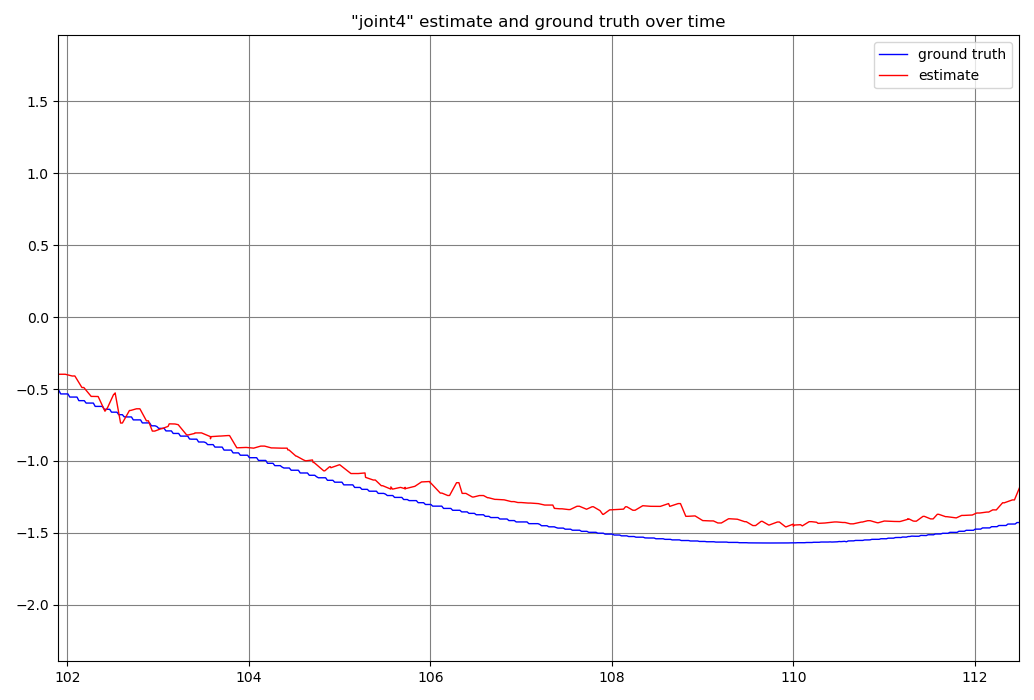
\includegraphics[width=0.7\textwidth]{plots/q2_1_j4_10sec.png}
\end{center}

\subsection{Description of target detection algorithm}
First, we detect the target in both of the camera feeds using 
template matching:
\begin{enumerate}
    \item \textbf{Isolate orange} elements using OpenCV's \texttt{inRange}
        method.
    \item 
        To distinguish between the target (sphere) and decoy
        (box), we perform \textbf{pattern matching} using OpenCV's
        \texttt{matchTemplate} method.
        We use a white circle with a darkened top and bottom
        so that the difference between the sphere and the box
        is more apparent.
    \item
        From the resulting image, we grab the position with the
        \textbf{least error} to determine the location of our target.
\end{enumerate}
Then, we combine both camera feeds to produce the 3D coordinates:
\begin{enumerate}
    \item
        Similar to the joints estimation algorithm, we assume that
        the camera feeds provide an orthogonal view across the
        entire plane.
    \item
        This simplification allows us to determine the coordinates:
        \[
            T = \begin{bmatrix} x \\ y \\ z \end{bmatrix} =
            \begin{bmatrix} 
                \text{cam}_2.x \\
                \text{cam}_1.x \\
                \frac{1}{2} (\text{cam}_1.y + \text{cam}_2.y)
            \end{bmatrix} 
        \]
\end{enumerate}

\subsection{Target detection plot}
\begin{center}
    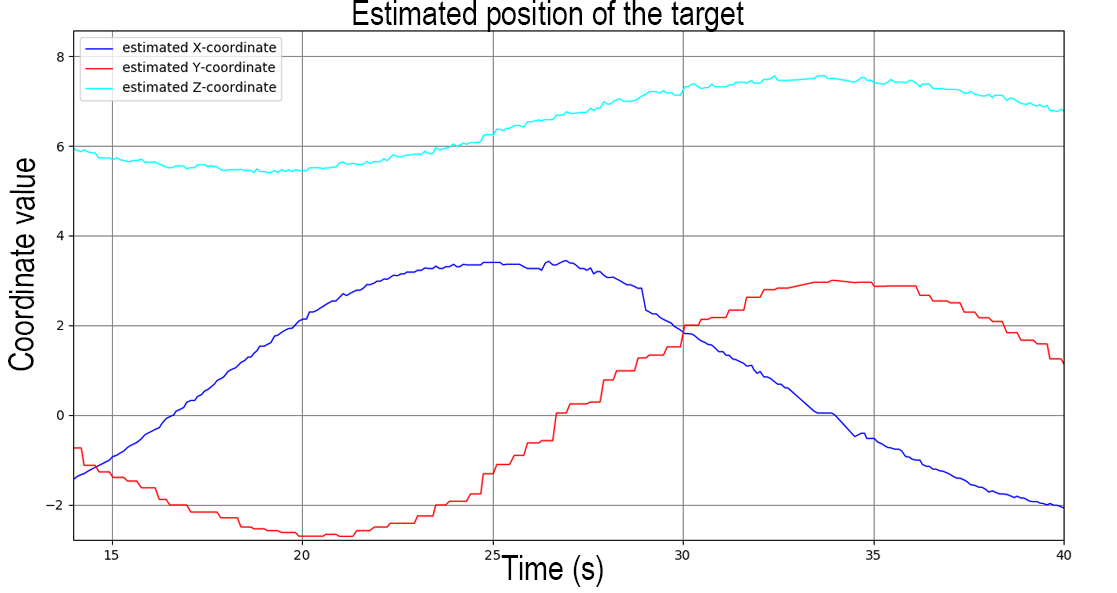
\includegraphics[width=0.8\textwidth]{plots/q2_2.png}
\end{center}
